\documentclass[11pt]{beamer}

\usetheme{Warsaw}
%\addtobeamertemplate{navigation symbols}{}{%
%    \usebeamerfont{footline}%
%    \usebeamercolor[fg]{footline}%
%    \hspace{1em}%
%    \insertframenumber/\inserttotalframenumber
%}

\beamertemplatenavigationsymbolsempty

\setbeamertemplate{footline}
{
  \leavevmode%
  \hbox{%
  \begin{beamercolorbox}[wd=.333333\paperwidth,ht=2.25ex,dp=1ex,center]{author in head/foot}%
    \usebeamerfont{author in head/foot} \hyperlink{Patrolling Games}{\inserttitle}
  \end{beamercolorbox}%
  \begin{beamercolorbox}[wd=.333333\paperwidth,ht=2.25ex,dp=1ex,center]{title in head/foot}%
    \usebeamerfont{title in head/foot}\insertauthor
  \end{beamercolorbox}%
  \begin{beamercolorbox}[wd=.333333\paperwidth,ht=2.25ex,dp=1ex,right]{date in head/foot}%
    \usebeamerfont{date in head/foot}\insertshortdate{}\hspace*{2em}
    \insertframenumber{} / \inserttotalframenumber\hspace*{2ex} 
  \end{beamercolorbox}}%
  \vskip0pt%
}
\setbeamertemplate{headline}{}
\usefonttheme[onlymath]{serif}

\usepackage{color}
\usepackage{xcolor}
\usepackage{tikz}
\usepackage{amsmath}
\usepackage{amssymb}
\usepackage{amsthm}
\usepackage{amsfonts}
\usepackage{graphicx}
\usepackage{mathtools}
\usepackage{wrapfig}
\usepackage{multirow}
\usepackage{comment}
\usepackage{natbib}
\usepackage{appendix}
\usepackage[utf8]{inputenc}
%\usepackage{floatrow}
%\usepackage{newfloat}
\usepackage{subcaption}
\usepackage{bm}
\usepackage{hyperref}

\usetikzlibrary{calc}
\usetikzlibrary{fit}
\usetikzlibrary{shapes.misc,calc, positioning, hobby, backgrounds}

\tikzset{cross/.style={cross out, draw=black, minimum size=2*(#1-\pgflinewidth), inner sep=0pt, outer sep=0pt},
%default radius will be 1pt. 
cross/.default={1pt}}


%\DeclarePairedDelimiter{\floor}{\lfloor}{\rightfloor}
%\DeclarePairedDelimiter{\ceil}{\lceil}{\rceil}

\newcommand{\halflength}{\ensuremath{\floor{\frac{m}{2}}}}
\newcommand{\floor}[1]{\left \lfloor #1 \right \rfloor}
\newcommand{\ceil}[1]{\left \lceil #1 \right \rceil}
\newcommand{\pospart}[1]{\left( #1 \right)_{+}}
\newcommand{\negpart}[1]{\left( #1 \right)_{-}}
\newcommand{\set}[2]{\left\{ #1 \, | \, #2 \right\}}

\newcommand{\oneline}[1]{\resizebox{\dimexpr\paperwidth - 3ex}{!}{#1}}

%\DeclareFloatingEnvironment[fileext=los,
 %   listname={List of Example Figures},
  %  name=Example Figure,
   % placement=tbhp,
    %within=section,]{examplefigure}

\author{Thomas Lowbridge}
\title{Patrolling Games}
%\setbeamercovered{transparent} 
%\setbeamertemplate{navigation symbols}{} 
%\logo{} 
\institute{University Of Nottingham} 
\date{December 13, 2017} 
%\subject{} 
\begin{document}

\hypertarget{Patrolling Games}{}
\begin{frame}
\titlepage
\end{frame}

%\begin{frame}
%\tableofcontents
%\end{frame}

\begin{frame}{Outline}

\begin{itemize}
\item Literature review
 \begin{itemize}
 \item Introduction to Game
  \begin{itemize}
  \item \hyperlink{Introduction to game: Pure game}{Pure game}
  \item \hyperlink{Introduction to game: Mixed game}{Mixed game}
  \end{itemize}
 \item Solved Graphs
  \begin{itemize}
  \item \hyperlink{Solved graphs: Hamiltonian graphs}{Hamiltonian graphs}
  \item \hyperlink{Solved graphs: Complete bipartite graphs}{Complete bipartite graph}
  \item \hyperlink{Solved graphs: Star graph}{Star graph}
  \item \hyperlink{Solved graphs: Line graph}{Line graph}
  \end{itemize}   
 \end{itemize}
\item \hyperlink{Problem with diametricstrategy}{Problem with line graph strategy}
\item \hyperlink{Correction of diametric line graph strategy}{Correction of line graph strategy}
\item \hyperlink{Extension of correction strategy}{Extension of correction strategy}
\item \hyperlink{Introduction to the elongated star}{Introduction to the elongated star}
\item \hyperlink{Future work}{Future work}
\end{itemize}
\end{frame}

\section[]{Introduction to Game: Pure game}
\hypertarget{Introduction to game: Pure game}{}
\begin{frame}{\insertsection}

A Patrolling game, $G=G(Q,T,m)$ is made of 3 major components
\begin{itemize}
\item A \textcolor{red}{Graph, $Q=(N,E)$}, made of nodes, $N$ ($|N|=n$), and a set of edges, $E$.
\item A \textcolor{red}{time horizon parameter, $T$} (with set $\mathcal{T}=\{0,1,...,T-1\}$).
\item An \textcolor{red}{attack time parameter, $m$}.
\end{itemize}

\pause

The game involves two players, the patroller and the attacker.
\begin{itemize}
\item The patroller's strategy is a walk (with waiting) on the graph, $W:\mathcal{T} \rightarrow  N$ .
\item The attacker's strategy is a node, $i$ and starting time, $\tau$ .
\end{itemize} 
The strategies are collected into the sets, $\mathcal{W}$ and $\mathcal{A}$ , for the patroller and attacker respectively, with some arbitrary labelling inside the set to form strategies $W_{i}$ and $A_{j}$.

\end{frame}

\begin{frame}{\insertsection}
The game is formulated as win-lose (a zero-sum game) with a payoff for the patroller of
\begin{align*}
P(W,(i,\tau))=\left\{ \begin{array}{l}
1 \text{  if  } i \in \left\{ W(\tau),W(\tau+1),...,W(\tau+m-1) \right\} ,\\
0 \text{  if  } i \notin \left\{ W(\tau),W(\tau+1),...,W(\tau+m-1) \right\} .\\
\end{array}\right.
\end{align*}
With a pure payoff matrix $\mathcal{P}=(P(W_{i},A_{j}))_{i \in \{ 1,...,|\mathcal{W}| \}, j \in \{ 1,...,|\mathcal{A}| \}}$
\end{frame}

\begin{frame}{\insertsection}
The game played on $Q$ as below with $m=3$ and $T=7$

\begin{center}
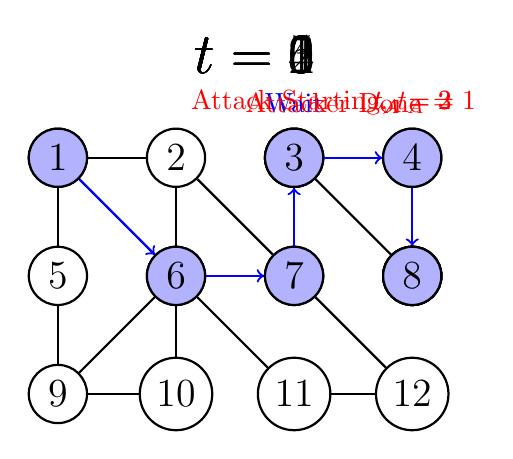
\begin{tikzpicture}[-,auto,node distance=1.5cm,
                    thick,main node/.style={circle,fill=white,draw,font=\sffamily\Large\bfseries}]

  \node[main node] (1) {$1$};
  \node[main node] (2) [right of=1] {$2$};
  \node[main node] (3) [right of=2]  {$3$};
  \node[main node] (4) [right of=3]  {$4$};
  \node[main node] (5) [below of=1]  {$5$};
  \node[main node] (6) [below of=2]  {$6$};
  \node[main node] (7) [below of=3]  {$7$};
  \node[main node] (8) [below of=4]  {$8$};
  \node[main node] (9) [below of=5]  {$9$};
  \node[main node] (10) [below of=6]  {$10$};
  \node[main node] (11) [below of=7] {$11$};
  \node[main node] (12) [below of=8] {$12$}; 

  \path[every node/.style={font=\sffamily}]
    (1) edge (2)
    (1) edge (5)
    (1) edge (6)
    (2) edge (6)
    (2) edge (7)
    (3) edge (7)
    (3) edge (4)
    (3) edge (8)
    (4) edge (8)
    (5) edge (9)
    (6) edge (7)
    (6) edge (10)
    (6) edge (11)
    (6) edge (9)
    (7) edge (12)
    (9) edge (10)
    (11) edge (12)
    ;

 %\node (GraphLabel) [shift={(0,1)}] at (1) {$Q$}; 

%Slide 2 (first animation)
  \visible<2>{
  \node (TimeLabel) [shift={(2.5,1.3)}] at (1) {\huge $t=0$};
  \node[main node,fill=blue!30] (1) at (1) {$1$};
  \path[->,color=blue] (1) edge (6); 
    }
%Slide 3
  \visible<3>{
   \node (TimeLabel) [shift={(2.5,1.3)}] at (1) {\huge $t=1$};
  \node[main node,fill=blue!30] (6) at (6) {$6$};
  \path[->,color=blue] (6) edge (7); 
    }
%Slide 4
  \visible<4>{
   \node (TimeLabel) [shift={(2.5,1.3)}] at (1) {\huge $t=2$};
  \node[main node,fill=blue!30] (7) at (7) {$7$};
  \path[->,color=blue] (7) edge (3);
  
  \node[main node,fill=red!30] (8) at (8) {$8$};
  \node[color=red] (Attacktimelabel) [shift={(-1,2.2)}] at (8) {Attack Starting, $t_{A}=1$};
    }
%Slide 5
  \visible<5>{
   \node (TimeLabel) [shift={(2.5,1.3)}] at (1) {\huge $t=3$};
  \node[main node,fill=blue!30] (3) at (3) {$3$};
  \node[color=blue] (WaitingLabel) [shift={(0,0.7)}] at (3) {Wait};
  
  \node[main node,fill=red!30] (8) at (8) {$8$};
  \node[color=red] (Attacktimelabel) [shift={(0,2.2)}] at (8) {$t_{A}=2$}; 
    }
%Slide 6
  \visible<6>{
   \node (TimeLabel) [shift={(2.5,1.3)}] at (1) {\huge $t=4$};
  \node[main node,fill=blue!30] (3) at (3) {$3$};
  \path[->,color=blue] (3) edge (4);
  
  \node[main node,fill=red!30] (8) at (8) {$8$};  
  \node[color=red] (Attacktimelabel) [shift={(0,2.2)}] at (8) {$t_{A}=3$};
    }
%Slide 7
  \visible<7>{
   \node (TimeLabel) [shift={(2.5,1.3)}] at (1) {\huge $t=5$};
  \node[main node,fill=blue!30] (4) at (4) {$4$};
  \path[->,color=blue] (4) edge (8); 
  
  \node[color=red] (Attacktimelabel) [shift={(-1,2.2)}] at (8) {Attacker Done};
    }    
%Slide 8
  \visible<8>{
   \node (TimeLabel) [shift={(2.5,1.3)}] at (1) {\huge $t=6$};
  \node[main node,fill=blue!30] (8) at (8) {$8$}; 
    }                 
\end{tikzpicture}

\end{center}
\only<1>{
\begin{itemize}
\item[] \textcolor{blue}{Patroller:} \textcolor{blue}{ $W(0)=1$ , $W(1)=6$ , $W(2)= 7$ , $W(3)=3$ , $W(4)=3$ , $W(5)=4$ , $W(8)= 8$}
\item[] \textcolor{red}{Attacker:} \textcolor{red}{$(8,2)$}
\end{itemize}
}
\only<8>
{
The attacker fails to catch the patroller, therefore the patroller loses (and the attacker wins) meaning a payoff of $0$ for the patroller (and $-1$ for the attacker).
}
\end{frame}

\section[]{Introduction to Game: Mixed game}
\hypertarget{Introduction to game: Mixed game}{}
\begin{frame}{\insertsection}
Both the patroller and attacker will play their pure(realised) strategies with certain probabilities, let $\bm{\pi}$ be a mixed strategy for the patroller and let $\bm{\phi}$ be a mixed strategy for the attacker. We collect these into the sets $\Pi$ and $\Phi$ for the patroller and attacker respectively.

Then the payoff for the patroller of this mixed game becomes
\begin{align*}
P(\bm{\pi} ,\bm{\phi})=\sum\limits_{i=1}^{|\mathcal{W}|} \sum\limits_{j=1}^{|\mathcal{I}|} \mathcal{P}_{i,j} \bm{\pi} _{i} \bm{\phi}_{j}
=\bm{\pi} \mathcal{P} \bm{\phi}
\end{align*}

By using the pure payoff as $1$ when capture occurs and $0$ otherwise, the mixed payoff is equivalent to the probability of capture.
\end{frame}

\begin{frame}{\insertsection}
\begin{block}{Mixed Nash equilibrium}
A choice of $\bm{\pi}^*$ and $\bm{\phi}^*$ is said to be in \textit{Nash equilibrium} if 
\begin{align*}
P(\bm{\pi}^*,\bm{\phi}^*) \geq P(\bm{\pi},\bm{\phi}^*) \quad \forall \bm{\pi} \in \Pi , \\
P(\bm{\pi}^*,\bm{\phi}^*) \geq P(\bm{\pi}^*,\bm{\phi}) \quad \forall \bm{\phi} \in \Phi .
\end{align*}
\end{block}
There will only be one Nash equilibrium, unless the patroller can guarantee capture.

We do this by searching for the games value, $$V(G) \equiv \max\limits_{\bm{\pi} \in \Pi} \min\limits_{\bm{\phi} \in \Phi} P(\bm{\pi},\bm{\phi})=\min\limits_{\bm{\phi} \in \Phi} \max\limits_{\bm{\pi} \in \Pi} P(\bm{\pi},\bm{\phi})$$
This is done by achieving both upper and lower bounds on the value of the game.
\end{frame}

\section[]{Solved graphs: Hamiltonian graphs}
\hypertarget{Solved graphs: Hamiltonian graphs}{}
\begin{frame}{\insertsection}

A graph is Hamiltonian if it is possible to find a cycle which visits every node exactly one (apart from the start/finish).

\begin{block}{Hamiltonian graphs}
A Hamiltonian graph has the value $V=\frac{m}{n}$
\end{block}

Two common Hamiltonian graphs are the Cyclic graph (of n nodes $C_{n}$) and the Complete graph (of n nodes $K_{n}$).
\begin{center}
\begin{figure}

\begin{tabular}{@{}c@{}}
  \begin{tabular}{c}
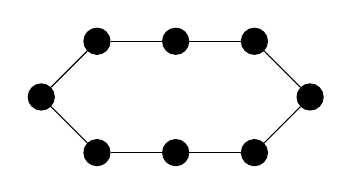
\begin{tikzpicture}[baseline=(current bounding box.north),-,auto,node distance=1cm,
                    main node/.style={circle,draw,fill=black,font=\sffamily\bfseries}]

  \node[main node] (1) {};
  \node[main node] (2) [above right of=1] {};
  \node[main node] (3) [right of=2] {};
  \node[main node] (4) [right of=3] {};
  \node[main node] (5) [below right of=4] {};
  \node[main node] (6) [below left of=5] {};
  \node[main node] (7) [left of=6] {};
  \node[main node] (8) [left of=7] {};
  

  \path[every node/.style={font=\sffamily}]
  (1) edge (2)
  (2) edge (3)
  (3) edge (4)
  (4) edge (5)
  (5) edge (6)
  (6) edge (7)
  (7) edge (8)
  (8) edge (1);

   
\end{tikzpicture}
     
      \\ \small $C_{8}$
  \end{tabular} \qquad
  \begin{tabular}{c}
  
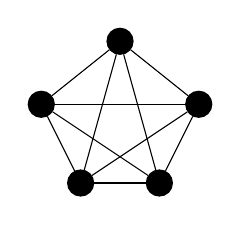
\begin{tikzpicture}[baseline=(current bounding box.north),-,auto,node distance=1cm,
                    main node/.style={circle,draw,fill=black,font=\sffamily\bfseries}]

  \node[main node] (1) {};
  \node[main node] (2) [shift={(1,-0.8)}] at (1) {};
  \node[main node] (3) [shift={(0.5,-1.8)}] at (1) {};
  \node[main node] (4) [shift={(-0.5,-1.8)}] at (1) {};
  \node[main node] (5) [shift={(-1,-0.8)}] at (1) {};

  

  \path[every node/.style={font=\sffamily}]
  (1) edge (2)
      edge (3)
      edge (4)
      edge (5)
  (2) edge (3)
      edge (4)
      edge (5)    
  (3) edge (4)
      edge (5)
  (4) edge (5);


   
\end{tikzpicture}

 \\ \small $K_{5}$
  \end{tabular} \\
\end{tabular}
\caption{Examples of Cyclic and Complete graphs}
\end{figure}
\end{center}



\end{frame}

\section[]{Solved graphs: Complete bipartite graphs}
\hypertarget{Solved graphs: Complete bipartite graphs}{}
\begin{frame}{\insertsection}

A bipartite graph is a graph made of two non-adjacent sets, the complete version has all connections.

\begin{block}{Complete bipartite graph}
A complete bipartite graph, $K_{a,b}$ as value
$V=\frac{m}{2 \max (a,b)}$
\end{block}

\begin{center}
\begin{figure}
\begin{tabular}{c}
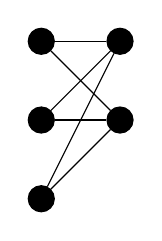
\begin{tikzpicture}[baseline=(current bounding box.north),-,auto,node distance=1cm,
                    main node/.style={circle,draw,fill=black,font=\sffamily\bfseries}]

  \node[main node] (1) {};
  \node[main node] (2) [below of=1] {};
  \node[main node] (3) [below of=2] {};
  \node[main node] (4) [right of=1] {};
  \node[main node] (5) [below of=4] {};

  

  \path[every node/.style={font=\sffamily}]
  (1) edge (4)
      edge (5)
  (2) edge (4)
      edge (5)    
  (3) edge (4)
      edge (5);

   
\end{tikzpicture}
\\ \small $K_{3,2}$
\end{tabular}
\caption{Example of a complete bipartite graph}
\end{figure}

\end{center}

\end{frame}

\section[]{Solved graphs: Star graph}
\hypertarget{Solved graphs: Star graph}{}
\begin{frame}{Solved graphs: Star graph}

The star graph,$S_{n}$, is $n$ nodes adjacent only to the centre. 

\begin{block}{Star graph}
The star $S_{n} \equiv K_{1,n}$ so has the value $V=\frac{m}{2n}$
\end{block}

\begin{center}
\begin{figure}
\begin{tabular}{c}
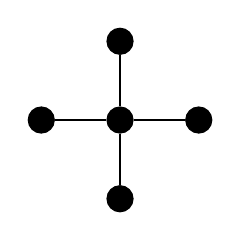
\begin{tikzpicture}[baseline=(current bounding box.north),-,auto,node distance=1cm,
                    main node/.style={circle,draw,fill=black,font=\sffamily\bfseries}]

  \node[main node] (1) {};
  \node[main node] (2) [above of=1] {};
  \node[main node] (3) [right of=1] {};
  \node[main node] (4) [below of=1] {};
  \node[main node] (5) [left of=1] {};

  

  \path[every node/.style={font=\sffamily}]
  (1) edge (2)
      edge (3)
      edge (4)
      edge (5);

   
\end{tikzpicture}
\\ \small $S_{4}$
\end{tabular}
\caption{Example of a star graph}
\end{figure}

\end{center}

\end{frame}

\section[]{Solved graphs: Line graph}
\hypertarget{Solved graphs: Line graph}{}
\begin{frame}{\insertsection}

The line graph, $L_{n}$, made of $n$ nodes each adjacent to two other nodes (apart from the ends)

\begin{block}{Line graph}
The line graph, $L_{n}$ has a value dependent on $(n,m)$
\begin{enumerate}
\item If $m > 2(n-1)$ then $V=1$.
\item If $n-1 < m \leq 2(n-1)$ then $V=\frac{m}{2(n-1)}$
\item If $m=2 , n\geq 3$ then $V=\frac{1}{\ceil{\frac{n}{2}}}$
\item If $m=n-1 \text{ or } m=n-2  \text{ and } m=2k \text{ for some } k \geq 2 $ then $V=\frac{1}{2}$
\item If $3 \leq m \leq n-3$ or  $m=n-2$ and $m=2k+1$ for some  $k \geq 1$ then $V=\frac{m}{m+n-1}$
\end{enumerate}
\end{block}
Note. The solution for $m=1$ is know for every graph as $V=\frac{1}{|N|}=\frac{1}{n}$, and if $m=n=2$ then we know $V=1$.
\end{frame}

\begin{frame}{\insertsection}

\begin{center}
\begin{figure}
\begin{tabular}{c}
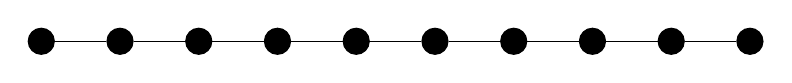
\begin{tikzpicture}[baseline=(current bounding box.north),-,auto,node distance=1cm,
                    main node/.style={circle,draw,fill=black,font=\sffamily\bfseries}]

  \node[main node] (1) {};
  \node[main node] (2) [right of=1] {};
  \node[main node] (3) [right of=2] {};
  \node[main node] (4) [right of=3] {};
  \node[main node] (5) [right of=4] {};
  \node[main node] (6) [right of=5] {};
  \node[main node] (7) [right of=6] {};
  \node[main node] (8) [right of=7] {};
  \node[main node] (9) [right of=8] {};
  \node[main node] (10) [right of=9] {};


  \path[every node/.style={font=\sffamily}]
  (1) edge (2)
  (2) edge (3)
  (3) edge (4)
  (4) edge (5)
  (5) edge (6)
  (6) edge (7)
  (7) edge (8)
  (8) edge (9)
  (9) edge (10);

   
\end{tikzpicture}
\\ \small $L_{10}$
\end{tabular}
\caption{Example of a line graph}
\end{figure}

\end{center}

\begin{columns}[onlytextwidth,T]
   \column{\dimexpr\linewidth-75mm-5mm}
    Regions are:  
    \begin{enumerate}
    \item $m>18$
    \item $9 < m \leq 18$
    \item $m=2$
    \item $m=9,8$
    \item $3 \leq m < 8$, $m=1$
    \end{enumerate}

      \column{75mm}
      \begin{minipage}{75mm}
      \begin{figure}
      \resizebox{\linewidth}{!}{
      % Created by tikzDevice version 0.10.1 on 2017-11-08 14:38:15
% !TEX encoding = UTF-8 Unicode
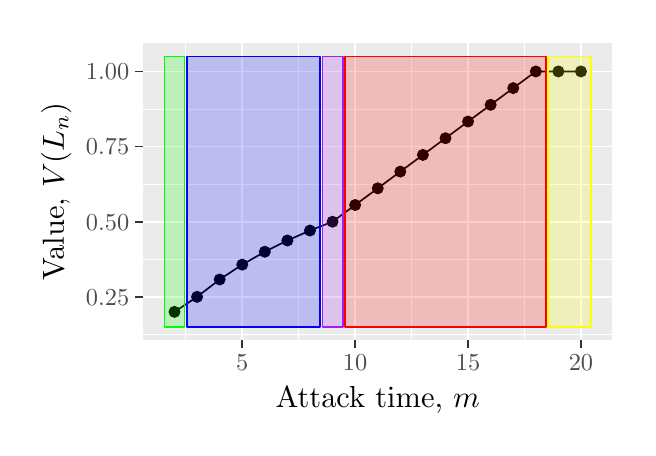
\begin{tikzpicture}[x=1pt,y=1pt]
\definecolor{fillColor}{RGB}{255,255,255}
\path[use as bounding box,fill=fillColor,fill opacity=0.00] (0,0) rectangle (216.81,144.54);
\begin{scope}
\path[clip] (  0.00,  0.00) rectangle (216.81,144.54);
\definecolor{drawColor}{RGB}{255,255,255}
\definecolor{fillColor}{RGB}{255,255,255}

\path[draw=drawColor,line width= 0.6pt,line join=round,line cap=round,fill=fillColor] (  0.00,  0.00) rectangle (216.81,144.54);
\end{scope}
\begin{scope}
\path[clip] ( 41.67, 31.53) rectangle (211.31,139.04);
\definecolor{fillColor}{gray}{0.92}

\path[fill=fillColor] ( 41.67, 31.53) rectangle (211.31,139.04);
\definecolor{drawColor}{RGB}{255,255,255}

\path[draw=drawColor,line width= 0.3pt,line join=round] ( 41.67, 33.70) --
	(211.31, 33.70);

\path[draw=drawColor,line width= 0.3pt,line join=round] ( 41.67, 60.85) --
	(211.31, 60.85);

\path[draw=drawColor,line width= 0.3pt,line join=round] ( 41.67, 88.00) --
	(211.31, 88.00);

\path[draw=drawColor,line width= 0.3pt,line join=round] ( 41.67,115.15) --
	(211.31,115.15);

\path[draw=drawColor,line width= 0.3pt,line join=round] ( 57.13, 31.53) --
	( 57.13,139.04);

\path[draw=drawColor,line width= 0.3pt,line join=round] ( 97.93, 31.53) --
	( 97.93,139.04);

\path[draw=drawColor,line width= 0.3pt,line join=round] (138.73, 31.53) --
	(138.73,139.04);

\path[draw=drawColor,line width= 0.3pt,line join=round] (179.53, 31.53) --
	(179.53,139.04);

\path[draw=drawColor,line width= 0.6pt,line join=round] ( 41.67, 47.28) --
	(211.31, 47.28);

\path[draw=drawColor,line width= 0.6pt,line join=round] ( 41.67, 74.43) --
	(211.31, 74.43);

\path[draw=drawColor,line width= 0.6pt,line join=round] ( 41.67,101.57) --
	(211.31,101.57);

\path[draw=drawColor,line width= 0.6pt,line join=round] ( 41.67,128.72) --
	(211.31,128.72);

\path[draw=drawColor,line width= 0.6pt,line join=round] ( 77.53, 31.53) --
	( 77.53,139.04);

\path[draw=drawColor,line width= 0.6pt,line join=round] (118.33, 31.53) --
	(118.33,139.04);

\path[draw=drawColor,line width= 0.6pt,line join=round] (159.13, 31.53) --
	(159.13,139.04);

\path[draw=drawColor,line width= 0.6pt,line join=round] (199.93, 31.53) --
	(199.93,139.04);
\definecolor{drawColor}{RGB}{0,0,0}
\definecolor{fillColor}{RGB}{0,0,0}

\path[draw=drawColor,line width= 0.4pt,line join=round,line cap=round,fill=fillColor] (191.77,128.72) circle (  1.96);

\path[draw=drawColor,line width= 0.4pt,line join=round,line cap=round,fill=fillColor] (199.93,128.72) circle (  1.96);

\path[draw=drawColor,line width= 0.4pt,line join=round,line cap=round,fill=fillColor] (118.33, 80.46) circle (  1.96);

\path[draw=drawColor,line width= 0.4pt,line join=round,line cap=round,fill=fillColor] (126.49, 86.49) circle (  1.96);

\path[draw=drawColor,line width= 0.4pt,line join=round,line cap=round,fill=fillColor] (134.65, 92.53) circle (  1.96);

\path[draw=drawColor,line width= 0.4pt,line join=round,line cap=round,fill=fillColor] (142.81, 98.56) circle (  1.96);

\path[draw=drawColor,line width= 0.4pt,line join=round,line cap=round,fill=fillColor] (150.97,104.59) circle (  1.96);

\path[draw=drawColor,line width= 0.4pt,line join=round,line cap=round,fill=fillColor] (159.13,110.62) circle (  1.96);

\path[draw=drawColor,line width= 0.4pt,line join=round,line cap=round,fill=fillColor] (167.29,116.66) circle (  1.96);

\path[draw=drawColor,line width= 0.4pt,line join=round,line cap=round,fill=fillColor] (175.45,122.69) circle (  1.96);

\path[draw=drawColor,line width= 0.4pt,line join=round,line cap=round,fill=fillColor] (183.61,128.72) circle (  1.96);

\path[draw=drawColor,line width= 0.4pt,line join=round,line cap=round,fill=fillColor] ( 53.05, 41.85) circle (  1.96);

\path[draw=drawColor,line width= 0.4pt,line join=round,line cap=round,fill=fillColor] (110.17, 74.43) circle (  1.96);

\path[draw=drawColor,line width= 0.4pt,line join=round,line cap=round,fill=fillColor] (102.01, 71.23) circle (  1.96);

\path[draw=drawColor,line width= 0.4pt,line join=round,line cap=round,fill=fillColor] ( 61.21, 47.28) circle (  1.96);

\path[draw=drawColor,line width= 0.4pt,line join=round,line cap=round,fill=fillColor] ( 69.37, 53.54) circle (  1.96);

\path[draw=drawColor,line width= 0.4pt,line join=round,line cap=round,fill=fillColor] ( 77.53, 58.91) circle (  1.96);

\path[draw=drawColor,line width= 0.4pt,line join=round,line cap=round,fill=fillColor] ( 85.69, 63.57) circle (  1.96);

\path[draw=drawColor,line width= 0.4pt,line join=round,line cap=round,fill=fillColor] ( 93.85, 67.64) circle (  1.96);

\path[draw=drawColor,line width= 0.6pt,line join=round] ( 53.05, 41.85) --
	( 61.21, 47.28) --
	( 69.37, 53.54) --
	( 77.53, 58.91) --
	( 85.69, 63.57) --
	( 93.85, 67.64) --
	(102.01, 71.23) --
	(110.17, 74.43) --
	(118.33, 80.46) --
	(126.49, 86.49) --
	(134.65, 92.53) --
	(142.81, 98.56) --
	(150.97,104.59) --
	(159.13,110.62) --
	(167.29,116.66) --
	(175.45,122.69) --
	(183.61,128.72) --
	(191.77,128.72) --
	(199.93,128.72);
\definecolor{drawColor}{RGB}{255,255,0}
\definecolor{fillColor}{RGB}{255,255,0}

\path[draw=drawColor,line width= 0.6pt,line join=round,fill=fillColor,fill opacity=0.20] (188.10, 36.42) rectangle (203.60,134.15);
\definecolor{drawColor}{RGB}{255,0,0}
\definecolor{fillColor}{RGB}{255,0,0}

\path[draw=drawColor,line width= 0.6pt,line join=round,fill=fillColor,fill opacity=0.20] (114.66, 36.42) rectangle (187.28,134.15);
\definecolor{drawColor}{RGB}{160,32,240}
\definecolor{fillColor}{RGB}{160,32,240}

\path[draw=drawColor,line width= 0.6pt,line join=round,fill=fillColor,fill opacity=0.20] (106.50, 36.42) rectangle (113.84,134.15);
\definecolor{drawColor}{RGB}{0,0,255}
\definecolor{fillColor}{RGB}{0,0,255}

\path[draw=drawColor,line width= 0.6pt,line join=round,fill=fillColor,fill opacity=0.20] ( 57.54, 36.42) rectangle (105.68,134.15);
\definecolor{drawColor}{RGB}{0,255,0}
\definecolor{fillColor}{RGB}{0,255,0}

\path[draw=drawColor,line width= 0.6pt,line join=round,fill=fillColor,fill opacity=0.20] ( 49.38, 36.42) rectangle ( 56.72,134.15);
\end{scope}
\begin{scope}
\path[clip] (  0.00,  0.00) rectangle (216.81,144.54);
\definecolor{drawColor}{gray}{0.30}

\node[text=drawColor,anchor=base east,inner sep=0pt, outer sep=0pt, scale=  0.88] at ( 36.72, 44.25) {0.25};

\node[text=drawColor,anchor=base east,inner sep=0pt, outer sep=0pt, scale=  0.88] at ( 36.72, 71.40) {0.50};

\node[text=drawColor,anchor=base east,inner sep=0pt, outer sep=0pt, scale=  0.88] at ( 36.72, 98.54) {0.75};

\node[text=drawColor,anchor=base east,inner sep=0pt, outer sep=0pt, scale=  0.88] at ( 36.72,125.69) {1.00};
\end{scope}
\begin{scope}
\path[clip] (  0.00,  0.00) rectangle (216.81,144.54);
\definecolor{drawColor}{gray}{0.20}

\path[draw=drawColor,line width= 0.6pt,line join=round] ( 38.92, 47.28) --
	( 41.67, 47.28);

\path[draw=drawColor,line width= 0.6pt,line join=round] ( 38.92, 74.43) --
	( 41.67, 74.43);

\path[draw=drawColor,line width= 0.6pt,line join=round] ( 38.92,101.57) --
	( 41.67,101.57);

\path[draw=drawColor,line width= 0.6pt,line join=round] ( 38.92,128.72) --
	( 41.67,128.72);
\end{scope}
\begin{scope}
\path[clip] (  0.00,  0.00) rectangle (216.81,144.54);
\definecolor{drawColor}{gray}{0.20}

\path[draw=drawColor,line width= 0.6pt,line join=round] ( 77.53, 28.78) --
	( 77.53, 31.53);

\path[draw=drawColor,line width= 0.6pt,line join=round] (118.33, 28.78) --
	(118.33, 31.53);

\path[draw=drawColor,line width= 0.6pt,line join=round] (159.13, 28.78) --
	(159.13, 31.53);

\path[draw=drawColor,line width= 0.6pt,line join=round] (199.93, 28.78) --
	(199.93, 31.53);
\end{scope}
\begin{scope}
\path[clip] (  0.00,  0.00) rectangle (216.81,144.54);
\definecolor{drawColor}{gray}{0.30}

\node[text=drawColor,anchor=base,inner sep=0pt, outer sep=0pt, scale=  0.88] at ( 77.53, 20.52) {5};

\node[text=drawColor,anchor=base,inner sep=0pt, outer sep=0pt, scale=  0.88] at (118.33, 20.52) {10};

\node[text=drawColor,anchor=base,inner sep=0pt, outer sep=0pt, scale=  0.88] at (159.13, 20.52) {15};

\node[text=drawColor,anchor=base,inner sep=0pt, outer sep=0pt, scale=  0.88] at (199.93, 20.52) {20};
\end{scope}
\begin{scope}
\path[clip] (  0.00,  0.00) rectangle (216.81,144.54);
\definecolor{drawColor}{RGB}{0,0,0}

\node[text=drawColor,anchor=base,inner sep=0pt, outer sep=0pt, scale=  1.10] at (126.49,  7.44) {Attack time, $m$};
\end{scope}
\begin{scope}
\path[clip] (  0.00,  0.00) rectangle (216.81,144.54);
\definecolor{drawColor}{RGB}{0,0,0}

\node[text=drawColor,rotate= 90.00,anchor=base,inner sep=0pt, outer sep=0pt, scale=  1.10] at ( 13.08, 85.29) {Value, $V(L_{n})$};
\end{scope}
\end{tikzpicture}
}
      \caption{Value of the line graph for varying $m$}
      \end{figure}
      \end{minipage}


    \end{columns}


\end{frame}

\begin{frame}{\insertsection}
Focusing in on $n-1 < m \leq 2(n-1)$. We will look at the strategies used to get the bounds $V \leq \frac{m}{2(n-1)}$ and $V \geq \frac{m}{2(n-1)}$.

\begin{itemize}
\item Patroller Strategy, $\bm{\pi}_{H}$, the embedded random Hamiltonian patrol.
\item Attacker Strategy, $\bm{\phi}_{D}$, the diametric attack.
\end{itemize}

\end{frame}

\begin{frame}{\insertsection}
An embedded random Hamiltonian patrol, $\bm{\pi}_{H}$, is made by `expanding' the line to be Hamiltonian (meaning every non-end node becomes two nodes). That is the patroller looks at $C_{2(n-1)}$ instead of $L_{n}$, then we get a bound of $V(C_{2(n-1)})=\frac{m}{2(n-1)}$. Now the patroller cannot do worse in $L_{n}$ than in $C_{2(n-1)}$, so a lower bound of $V \geq \frac{m}{2(n-1)} $ is achieved. In the line graph this is also known as oscillation.

\begin{figure}
\begin{center}
\resizebox{\textwidth}{!}{
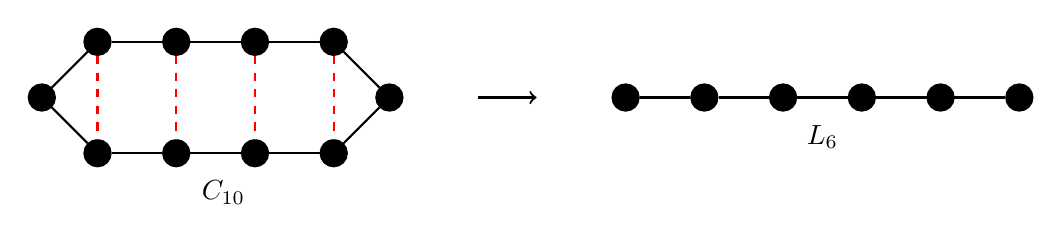
\begin{tikzpicture}[baseline=(current bounding box.north),-,auto,node distance=1cm,
                    thick,main node/.style={circle,draw,fill=black,font=\sffamily\bfseries}]

  \node[main node] (1) {};
  \node[main node] (2) [above right of=1] {};
  \node[main node] (3) [right of=2] {};
  \node[main node] (4) [right of=3] {};
  \node[main node] (5) [right of=4] {};
  \node[main node] (6) [below right of=5] {};
  \node[main node] (7) [below right of=1] {};
  \node[main node] (8) [right of=7] {};
  \node[main node] (9) [right of=8] {};
  \node[main node] (10) [right of=9] {};
  
  \node (P1) [right of=6] {};
  \node (P2) [right of=P1] {};
  
  \node[main node] (a) [right of=P2] {};
  \node[main node] (b) [right of=a] {};
  \node[main node] (c) [right of=b] {};
  \node[main node] (d) [right of=c] {};
  \node[main node] (e) [right of=d] {};
  \node[main node] (f) [right of=e] {};
  
  \draw[->] (P1) edge (P2);
  

  \path[every node/.style={font=\sffamily}]
    (1) edge  (2)
    edge (7)
    (2) edge (3)
    (3) edge (4)
    (4) edge (5)
    (5) edge (6)
    (6) edge (10)
    (7) edge (8)
    (8) edge (9)
    (9) edge (10)
    (a) edge (b)
    (b) edge (c)
    (c) edge (d)
    (d) edge (e)
    edge (f);
    
     \path[dashed,thick,red,every node/.style={font=\sffamily}]
    (2) edge  (7)
    (3) edge (8)
    (4) edge  (9)
    (5) edge  (10);
    
  
\node [shift={(0.6,-0.5)}] at (8) {$C_{10}$};
\node [shift={(0.5,-0.5)}] at (c) {$L_{6}$};   
\end{tikzpicture}
}
\end{center}
\caption{$C_{10}$ can be simplified to $L_{6}$ by node identifying.}
\end{figure}
\end{frame}

\begin{frame}{\insertsection}
Let $d(i,i')$ is the distance between nodes $i$ and $i'$ with the distance measured by the minimum number of edges.

\begin{definition}[Graph Diameter]
The diameter of a graph $Q$ is definded by $\bar{d}=\max\limits_{i,i' \in N} d(i,i')$ . The node pairs satisfying this are called diametrical.
\end{definition}

A diametric attack, $\bm{\phi}_{D}$ is made by attacking the pair of diametric nodes $1$ and $n$ (the ends), starting with equal probability at every available star time. It is stated to give a bound of $V \leq \min\{\frac{1}{2},\frac{m}{2(n-1)}\}= \left\{
\begin{array}{l} 
\frac{1}{2} \text{, if } m<n-1 \\
\frac{m}{2(n-1)} \text{, if } n-1 \leq m \leq 2(n-1),
\end{array}
\right.$ however....
\end{frame}

\section[]{Problem with the diametric strategy}
\hypertarget{Problem with diametric strategy}{}
\begin{frame}{\insertsection}

In the region of $n-1 \leq m \leq 2(n-1)$ the proposed bound is $V \leq \frac{m}{2(n-1)}$. However a simple counter shows this to be false.
\newline
\newline
\textbf{Counter-example.}
Consider $L_{5}$ with $T=m=5$ , then the patroller only needs to walk between the end nodes to win.
\begin{center}
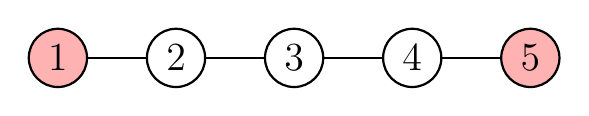
\begin{tikzpicture}[-,auto,node distance=1.5cm,
                    thick,main node/.style={circle,fill=white,draw,font=\sffamily\Large\bfseries}]

  \node[main node,fill=red!30] (1) {$1$};
  \node[main node] (2) [right of=1] {$2$};
  \node[main node] (3) [right of=2]  {$3$};
  \node[main node] (4) [right of=3]  {$4$};
  \node[main node,fill=red!30] (5) [right of=4] {$5$};

  \path[every node/.style={font=\sffamily}]
    (1) edge (2)
    (2) edge (3)
    (3) edge (4)
    (4) edge (5)
    ;
\end{tikzpicture}
\end{center}
The walk $\{ 1,2,3,4,5 \}$ guarantee's the capture of all attacks made.

\end{frame}

\begin{frame}{\insertsection}

\textbf{Example.}
Consider $L_{31}$ with $m=45$

\begin{figure}
%\includegraphics[scale=0.4]{DiametricAttack(m_45,d_30)1.png}
\resizebox{0.95\linewidth}{!}{
\input{DiametricAttack(m_45,d_30).tex}}
\caption{Best Upper Bound achievable under the diametric strategy}
\end{figure}

\end{frame}

\begin{frame}{\insertsection}

The problem is under the diametric attack, a patroller can catch
\tiny


\begin{align*}
&m-\bar{d}+\pospart{m \times (\floor{\frac{T-2m+1}{\bar{d}}}+1)} +  \pospart{T-(m-1+(\floor{\frac{T-2m+1}{\bar{d}}}+1)\bar{d})} +  \\
&\hspace{75pt} \pospart{T-(m-1+(\floor{\frac{T-2m+1}{\bar{d}}}+2)\bar{d})}
\end{align*}

\normalsize
attacks. From this we can get

\begin{lemma}[Condition on $T$ for bound to hold]
When $T=m-1+(k+1)(n-1)$ for some $k \in \mathbb{N}_{0}$ then the diametric bound holds. Otherwise as $T \rightarrow \infty$ then the diametric bound, $V \leq \frac{m}{2(n-1)}$, holds.
\end{lemma}

\end{frame}


\section[]{Correction to diametric line strategy}
\hypertarget{Correction to line graph strategy}{}
\begin{frame}{\insertsection}
We propose a solution to the problem, by limiting the time

\begin{definition}[Time limited diametric attack]
When $T \geq m+n-2$ we have the \textit{time limited diametric attack} (on the line) strategy is for the attacker to attack at both ends of the line with equal probability for starting times $0,1,...,n-2$
\end{definition}

This restriction to the attacking time guarantees to get the upper bound of $V \leq \frac{m}{2(n-1)}$.
\end{frame}

\section[]{Extension to time limited diametric strategy}
\hypertarget{Extension of correction strategy}{}
\begin{frame}{\insertsection}

\begin{definition}[Time limited diametric attack]
When $T \geq m-1+\bar{d}$ we have the \textit{time limited diametric attack} strategy is for the attacker to attack at both ends of the line with equal probability for starting times $\tau,\tau +1,...,\tau + \bar{d}-1$ (for a chosen initial $\tau$).
\end{definition}

\begin{lemma}[Time limited diametric bound]
When $T \geq m-1 +\bar{d}$ the attacker can get the bound
$$V \leq \dfrac{m}{2\bar{d}}.$$
\end{lemma}

\end{frame}


\begin{frame}{\insertsection}
\begin{columns}[onlytextwidth]
   \column{\dimexpr\linewidth-40mm-5mm}
\begin{definition}[Polygonal attack]
A \textit{$d$-polygonal attack} is an attack at a set of nodes $D= \set{i \in N}{ d(i,j)=d , \forall j \in D}$ at the time intervals $\tau,\tau+1,...,\tau+d-1$ (for a chosen initial $\tau$) all equally probable.
\end{definition}

\begin{lemma}[Polygonal bound]
When $T \geq m+d-1$ and a set $D$ as in the $d$-polygonal attack exists, the value has an upper bound of $V \leq \max \{ \frac{1}{|D|} , \frac{m}{|D|d} \}$ .
\end{lemma}

      \column{40mm}
      \begin{minipage}{40mm}
      \textbf{Example.}
\begin{figure}
\begin{center}
\resizebox{\linewidth}{!}{
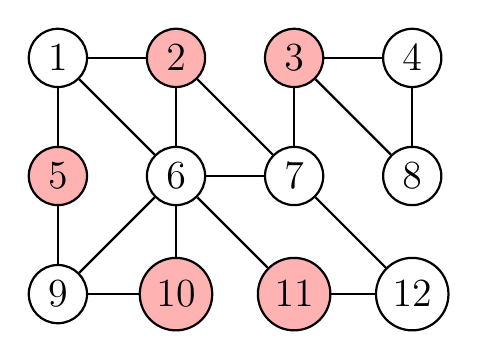
\begin{tikzpicture}[-,auto,node distance=1.5cm,
                    thick,main node/.style={circle,fill=white,draw,font=\sffamily\Large\bfseries}]

  \node[main node] (1) {$1$};
  \node[main node,fill=red!30] (2) [right of=1] {$2$};
  \node[main node,fill=red!30] (3) [right of=2]  {$3$};
  \node[main node] (4) [right of=3]  {$4$};
  \node[main node,fill=red!30] (5) [below of=1]  {$5$};
  \node[main node] (6) [below of=2]  {$6$};
  \node[main node] (7) [below of=3]  {$7$};
  \node[main node] (8) [below of=4]  {$8$};
  \node[main node] (9) [below of=5]  {$9$};
  \node[main node,fill=red!30] (10) [below of=6]  {$10$};
  \node[main node,fill=red!30] (11) [below of=7] {$11$};
  \node[main node] (12) [below of=8] {$12$}; 

  \path[every node/.style={font=\sffamily}]
    (1) edge (2)
    (1) edge (5)
    (1) edge (6)
    (2) edge (6)
    (2) edge (7)
    (3) edge (7)
    (3) edge (4)
    (3) edge (8)
    (4) edge (8)
    (5) edge (9)
    (6) edge (7)
    (6) edge (10)
    (6) edge (11)
    (6) edge (9)
    (7) edge (12)
    (9) edge (10)
    (11) edge (12)
    ;
\end{tikzpicture}}    
\end{center}
\caption{$2$-polygonal attack on $D=\{2,3,5,10,11  \}$ }
\end{figure}
Giving $V \leq \max\{\frac{1}{5},\frac{m}{10} \}$.
      \end{minipage}


    \end{columns}


\end{frame}

\section[]{Introduction to the elongated star}
\hypertarget{Introduction to the elongated star}{}
\begin{frame}{\insertsection}


We now wish to integrate features of a star into a line.
We will form the elongated star $S_{n}^{k}$. We will use the labelling as below

\begin{figure}
\begin{center}
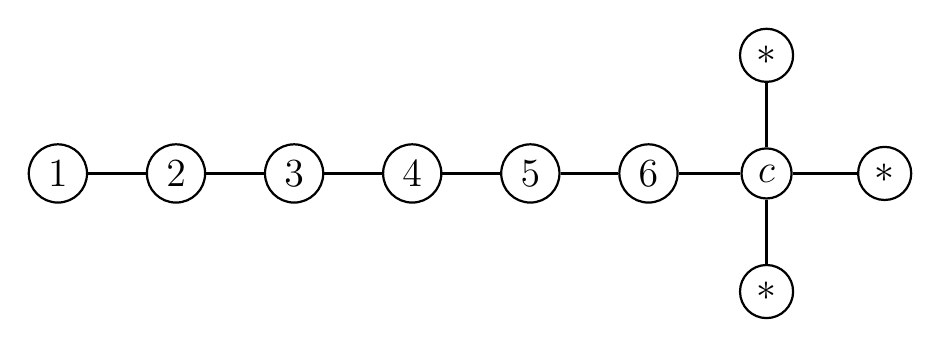
\begin{tikzpicture}[-,auto,node distance=1.5cm,
                    thick,main node/.style={circle,draw,font=\sffamily\Large\bfseries}]

  \node[main node] (1) {$1$};
  \node[main node] (2) [right of=1] {$2$};
  \node[main node] (3) [right of=2] {$3$};
  \node[main node] (4) [right of=3] {$4$};
  \node[main node] (5) [right of=4] {$5$};
  \node[main node] (6) [right of=5]  {$6$};
  \node[main node] (7) [right of=6]  {$c$};
  \node[main node] (8) [right of=7]  {$*$};
  \node[main node] (9) [above of=7]  {$*$};
  \node[main node] (10) [below of=7]  {$*$};
  

  \path[every node/.style={font=\sffamily}]
    (1) edge  (2)
    (2) edge (3)
    (3) edge (4)
    (4) edge (5)
    (5) edge (6)
    (6) edge (7)
    (7) edge (8)
     edge (9)
     edge (10);
\end{tikzpicture}
\end{center}
\caption{Labeling on the graph $S_{4}^5$.}
\end{figure}

\end{frame}

\begin{frame}{\insertsection}

\begin{definition}[Random Oscillation]
The \textit{Oscillation} on $S_{n}^{k}$ is any embedded Hamiltonian Patrol on $C_{2(n+k)}$.

The \textit{Random Oscillation} on $S_{n}^{k}$ is the embedded Random Hamiltonian Patrol on $C_{2(n+k)}$.
\end{definition}

\begin{figure}
\begin{center}
\resizebox{\textwidth}{!}{
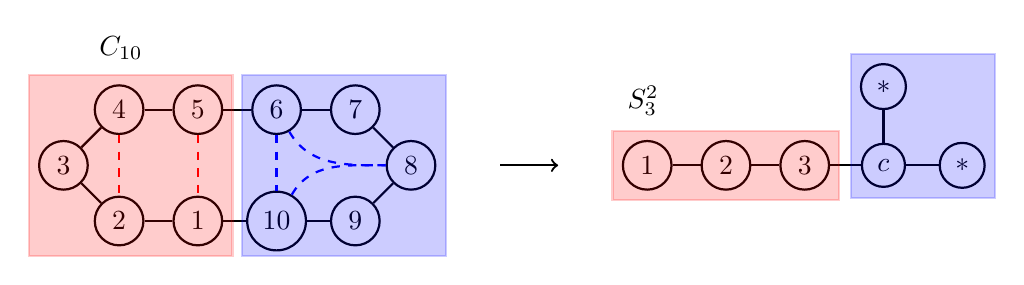
\begin{tikzpicture}[baseline=(current bounding box.north),-,auto,node distance=1cm,
                    thick,main node/.style={circle,draw,font=\sffamily\bfseries}]

  \node[main node] (1) {$3$};
  \node[main node] (2) [above right of=1] {$4$};
  \node[main node] (3) [right of=2] {$5$};
  \node[main node] (4) [right of=3] {$6$};
  \node[main node] (5) [right of=4] {$7$};
  \node[main node] (6) [below right of=5] {$8$};
  \node[main node] (7) [below right of=1] {$2$};
  \node[main node] (8) [right of=7] {$1$};
  \node[main node] (9) [right of=8] {$10$};
  \node[main node] (10) [right of=9] {$9$};
  
  \node (P1) [right of=6] {};
  \node (P2) [right of=P1] {};
  
  \node[main node] (a) [right of=P2] {$1$};
  \node[main node] (b) [right of=a] {$2$};
  \node[main node] (c) [right of=b] {$3$};
  \node[main node] (d) [right of=c] {$c$};
  \node[main node] (e) [right of=d] {$*$};
  \node[main node] (f) [above of=d] {$*$};
  
  \draw[->] (P1) edge (P2);
  

  \path[every node/.style={font=\sffamily}]
    (1) edge  (2)
    edge (7)
    (2) edge (3)
    (3) edge (4)
    (4) edge (5)
    (5) edge (6)
    (6) edge (10)
    (7) edge (8)
    (8) edge (9)
    (9) edge (10)
    (a) edge (b)
    (b) edge (c)
    (c) edge (d)
    (d) edge (e)
    edge (f);
    
     \path[dashed,red,every node/.style={font=\sffamily}]
    (2) edge  (7)
    (3) edge (8);
    
    \path[dashed,blue,every node/.style={font=\sffamily}]
    (4) edge  (9);
    
    \path[dashed,blue,out=-60,in=180,every node/.style={font=\sffamily}]
    (4) edge (6);
    
    \path[dashed,blue,out=60,in=180,every node/.style={font=\sffamily}]
    (9) edge (6);
  
  \node (Box1) [draw,thick,fit=(1) (2) (3) (7) (8),fill,red,opacity=0.2] {};
  \node (Box2) [draw,thick,fit=(4) (5) (6)  (10),fill,blue,opacity=0.2] {};
  
  \node (Box3) [draw,thick,fit=(a) (b) (c),fill,red,opacity=0.2] {}; 
  \node (Box4) [draw,thick,fit=(d) (e) (f),fill,blue,opacity=0.2] {};   
  
\node [left=0.5cm,above=0.5cm,text width=0.5cm] at (2) {$C_{10}$};
\node [left=0.5cm,above=0.5cm,text width=0.5cm] at (a) {$S_{3}^{2}$};   
\end{tikzpicture}
}
\end{center}
\caption{$C_{10}$ can be simplified to $S_{3}^{2}$ by node identifying.}
\end{figure}

\end{frame}

\begin{frame}{\insertsection}
\begin{lemma}
For $m < 2(n+k)$ following the Random Oscillation,
$$V(S_{n}^{k}) \geq V(C_{2(n+k)})=\frac{m}{2(n+k)}$$
and if $m \geq 2(n+k)$ then $V(S_{n}^{k})=1$, achieved by any Oscillation.
\end{lemma}
\end{frame}

\begin{frame}{\insertsection}
We adapt the time limited diametric attack to the time-delayed attack.

\begin{definition}[Time-delayed attack]
Let the \textit{time-delayed attack}, be the attack that attacks at the extended node labelled $1$ with probability $\frac{k+1}{n+k}$ and a particular normal node labelled $*$ with probability $\frac{1}{n+k}$.

If node $1$ is chosen have the attack choose probability intervals with equal probability starting attacks at $\tau, \tau+1,...,\tau+2k+1$. If a $*$ node is chosen start the attacks at the times $\tau+k,\tau+k+1$ with equal probability.
\end{definition}

\begin{figure}
\begin{center}
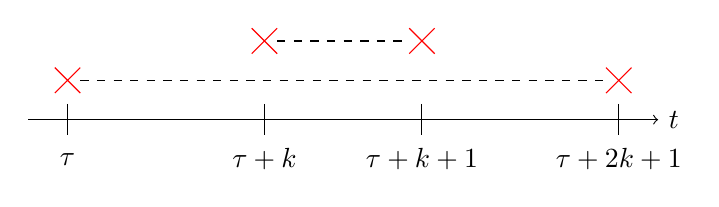
\begin{tikzpicture}
 \draw[->] (-4,0) -- (4,0);
 \node (timelabel) [shift={(0.2,0)}] at (4,0) {$t$};
 
 
 \draw (-3.5,0.2) -- (-3.5,-0.2);
 \draw (3.5,0.2) -- (3.5,-0.2);
 
 \node (labelc1) at (-3.5,-0.5) {$\tau$};
 \node (labelc2) at (3.5,-0.5) {$\tau+2k+1$};
 
 \node[cross=5pt,red] (c1) at (-3.5,0.5) {};
 \node[cross=5pt,red] (c2) at (3.5,0.5) {};
 \draw[dashed] (c1) -- (c2);
 
 \draw (-1,0.2) -- (-1,-0.2);
 \draw (1,0.2) -- (1,-0.2);
 
  \node (labelc3) at (-1,-0.5) {$\tau+k$};
 \node (labelc4) at (1,-0.5) {$\tau+k+1$};
 
 \node[cross=5pt,red] (c3) at (-1,1) {};
 \node[cross=5pt,red] (c4) at (1,1) {};
 \draw[dashed] (c3) -- (c4);

\end{tikzpicture}
\end{center}
\end{figure}



\end{frame}

\section[]{Future Work}
\hypertarget{Future work}{}
\begin{frame}{\insertsection}

\begin{itemize}
\item Look at analysing different types of Polygonal attacks
\end{itemize}

\end{frame}


\end{document}